\documentclass[letterpaper,12pt]{article}
\usepackage[spanish]{babel}
\spanishdecimal{.}
\selectlanguage{spanish}
\usepackage[spanish,onelanguage,ruled]{algorithm2e}
\usepackage[utf8]{inputenc}
\usepackage{graphicx}
\usepackage{caption}
\usepackage{subcaption}
\usepackage[top=2cm, bottom=2cm, left=2cm, right=2cm]{geometry}
\usepackage{hyperref}
\usepackage{verbatim}
\usepackage{amssymb}
\usepackage{mathtools}
\newcommand\ddfrac[2]{\frac{\displaystyle #1}{\displaystyle #2}}
\DeclareMathOperator{\atantwo}{atan2}

\title{Práctica 6  \\ Control de posición y seguimiento de rutas}
\author{Laboratorio de Bio-Robótica}
\date{Robots Móviles y Agentes Inteligentes}
\begin{document}
\renewcommand{\tablename}{Tabla}
\maketitle
\section*{Objetivos}
\begin{itemize}
\item Implementar un control de posición y de seguimiento de rutas. 
\item Probar el control tanto en simulación como en el robot real.
\item Utilizar como referencia la ruta calculada en la práctica 5.
\end{itemize}

\section{Marco Teórico}
\subsection{Modelo cinemático del robot}
Considérese un robot diferencial como el de la figura \ref{fig:Coords} en el que la configuración está dada por tres valores $\left[x_r, y_r, \theta_r\right]$. Considerando sólo la parte cinemática y asumiendo que no existe deslizamiento en las llantas, el modelo del robot está dado por
\begin{eqnarray}                                                                                                                        
\dot{x_r} &=& \frac{v_l + v_r}{2}\cos\theta_r\label{eq:Kinematic1}\\                                                                        
\dot{y_r} &=& \frac{v_l + v_r}{2}\sin\theta_r\\                                                                                             
\dot{\theta_r} &=& \frac{v_r - v_l}{L}\label{eq:Kinematic3}                                                                               
\end{eqnarray}
donde $v_l$ y $v_r$ son las velocidades lineales de las llantas izquierda y derecha respectivamente, consideradas como señales de entrada, y $L$ es el diámetro del robot medido de eje a eje de las llantas. Se considera que el centro del robot está en el centro de dicho eje.

Nótese que no se está modelando la parte dinámica del robot, esto es, se considera que el estado del robot está dado por los mismos tres valores $\left[x_r, y_r, \theta_r\right]$ y que las velocidades de las llantas se pueden fijar de manera arbitraria. En realidad, esto no sucede así. La verdadera señal de control es el voltaje que se fija en las terminales de los motores, sin embargo, se puede considerar que las dinámicas tanto eléctrica como mecánica de dichos motores son lo suficientemente rápidas para suponer que un voltaje en el motor se reflejará \textit{rápidamente} en una velocidad angular.

Para lidiar con las incertidumbres que provocan todas estas dinámicas no modeladas y con perturbaciones, se implementará un control realimentado.
\begin{figure}
\centering
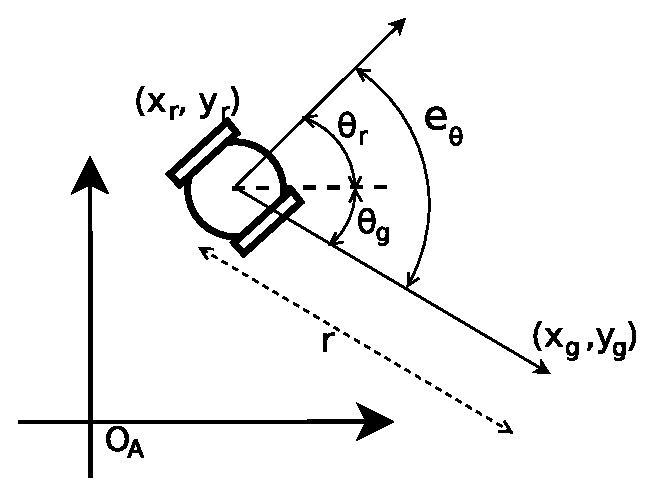
\includegraphics[width=0.5\textwidth]{Figures/GoalPose.eps}
\caption{Posición del robot y posición deseada.}
\label{fig:Coords}
\end{figure}

\subsection{Control de posición}
El objetivo del control es diseñar las señales $v_l$ y $v_r$ de modo que se garantice que el robot llegue a la posición $\left(x_g, y_g\right)$ aun en presencia de incertidumbres (como las dinámicas no modeladas) y perturbaciones. En esta práctica se implementarán dos leyes de control, pero antes es necesario definir un par de variables. 

Considérese el esquema de la figura \ref{fig:Coords}. El ángulo deseado $\theta_g$ corresponde al ángulo del vector de error de posición $\left[x_g - x_r, y_g - y_r\right]$, esto es
\[\theta_g = \atantwo\left(y_g - y_r, x_g - x_r\right)\]
de donde se define el error de ángulo
\[e_{\theta} = \theta_g - \theta_r = \atantwo\left(y_g - y_r, x_g - x_r\right) - \theta_r\]
El error de distancia $r$ es simplemente la magnitud del vector de error de posición:
\[r= \left[\left(x_g - x_r\right) + \left(y_g - y_r\right)\right]^{1/2}\]
En la primera ley de control las velocidades se calculan tomando en cuenta tanto el error de posición como el de ángulo:
\begin{eqnarray}
v_{l} &=& -k_{\theta}e_{\theta} + k_d r e^{-\psi e_{\theta}^2}\label{eq:Control11}\\
v_{r} &=&  k_{\theta}e_{\theta} + k_d r e^{-\psi e_{\theta}^2}\label{eq:Control12}
\end{eqnarray}
Nótese que los primeros términos tienen igual magnitud pero signo opuesto, lo que provoca una velocidad angular que es proporcional al error de ángulo. Los segundos términos, al tener el mismo signo y misma magnitud, provocan una velocidad lineal que es proporcional al error de distancia, es decir, el robot se irá deteniendo conforme se acerque al punto meta. La exponencial sirve para hacer pequeña la velocidad lineal cuando el error de ángulo es grande, es decir, este término logra que el robot comience a avanzar hasta que esté apuntando en la dirección correcta.

En esta ley de control se tienen tres parámetros de diseño: $k_{\theta}>0$, $k_d>0$ y $\psi>0$. Las dos primeras determinan la rapidez con que el robot girará y avanzará hacia el punto meta. La tercera es muy importante. Un valor de $\psi$ muy grande hará que la velocidad lineal decrezca muy rápido cuando crece el error de ángulo, es decir, el robot comenzará a avanzar hasta que esté apuntando casi sin error hacia la meta. Por el contrario, una $\psi$ muy pequeña hará que el robot describa curvas muy grandes.  

La segunda ley de control sólo toma en cuenta el error de ángulo:
\begin{eqnarray} 
v_{l} &=& v_{max}e^{-\frac{e_{\theta}^{2}}{\alpha}} + 
\frac{D}{2}\omega_{max}\left(\frac{2}{1+e^{-\frac{e_{\theta}}{\beta}}}-1\right)\label{eq:Control21}\\
v_{r} &=& v_{max}e^{-\frac{e_{\theta}^{2}}{\alpha}} -
\frac{D}{2}\omega_{max}\left(\frac{2}{1+e^{-\frac{e_{\theta}}{\beta}}}-1\right)\label{eq:Control22}
\end{eqnarray}
En estas ecuaciones se tienen cuatro parámetros de diseño: $v_{max}$ y $\omega_{max}$ son las velocidades lineales y angulares máximas respectivamente que el robot alcanzará durante su movimiento. La constante $\alpha$ tiene una función parecida a la $\psi$ en las ecuaciones (\ref{eq:Control11})-(\ref{eq:Control12}), solo que en este caso, al estar dividiendo, una $\alpha$ más pequeña provocará un descenso más pronunciado en la magnitud de la velocidad lineal. El valor de $\beta$ determina qué tanto decrece la velocidad angular conforme decrece el error de ángulo. 

Esta ley de control tiene la desventaja de que sólo depende del error de ángulo, es decir, que el robot no disminuye su velocidad conforme se acerca al punto meta, como en (\ref{eq:Control11})-(\ref{eq:Control12}). Esto provoca que el robot presente fuertes oscilaciones cuando se encuentra en una región pequeña alrededor del punto meta.

Hay dos formas de abordar este problema. La más sencilla consiste en ejecutar la ley de control sólo si la distancia $d=\sqrt{(x_g - x_r)^2 + (y_g - y_r)^2}$ es mayor que una tolerancia, es decir:

\[
  \left[\begin{tabular}{c}$v_l$ \\ $v_r$ \end{tabular}\right] =
  \begin{cases}
    
    \end{cases}
\]

\subsection{Perfil de velocidad}

\section{Tareas}

\subsection{Prerrequisitos}
Antes de continuar, actualice el repositorio y recompile:
\begin{verbatim}
   cd ~/RoboticsCourses
   git pull origin master
   cd catkin_ws
   catkin_make
\end{verbatim}

\subsection{Nodo para el control de bajo nivel}
Hacer un nodo de ROS que ...
La primera ley de control se debe usar para realizar movimientos del tipo move.
La segunda se debe usar para seguir trayectorias, calculadas con A* y con un perfil de velocidad. 

\subsection{Pruebas experimentales y en simulación}
Launch para simulación. Launch para pruebas reales.

\section{Evaluación}
\begin{itemize}
\item El control se probará siguiendo la ruta calculada en la práctica 5. 
\item Las constantes de las leyes de control deben ser fácilmente modificables. 
\item El código debe estar ordenado.
\item \textbf{Importante: } Si el alumno no conoce su código, NO se contará la práctica.
\end{itemize}

\end{document}